\newpage
\section*{Додаток А. Ілюстрації}
\setlength{\parindent}{0cm}
\addcontentsline{toc}{section}{Додаток А. Ілюстрації}
\begin{tikzpicture}
\makeatletter
\tikzset{
 circle connection bar/.style={rectangle,draw=\tikz@concept@color,every circle connection bar},
 every concept/.append style={minimum size=0cm, color=black, fill=white},
 concept/.style={circle,draw=\tikz@concept@color,every concept},
 every node/.append style={concept}
} \makeatother
\path[
 mindmap,
 scale=0.8,
 level 1 concept/.append style={sibling angle=120},
 level 2 concept/.append style={sibling angle=60},
 level 3 concept/.append style={sibling angle=30},
 level 4 concept/.append style={sibling angle=32,text width=1cm},
 sys/.style={concept, font=\footnotesize},
]
node [sys] {Система обліку платних курсів\\із підтримкою самостійного запису слухачів через мережу Інтернет} [clockwise from=210]
 child {
  node {Вхідний потік} [clockwise from=330]
   child { node {Хто?} [clockwise from=340]
    child { node {Оператори} }
    child { node [text width=1.4cm] {Адміністратор} }
    child [sibling angle=32] { node {Слухачі} [clockwise from=330]
     child { node {Студенти} }
     child { node {Сторонні} }
    }
   }
   child { node {Що?} [clockwise from=320]
    child { node {Дані слухачів} }
    child { node {Курси} }
    child { node {Дані викладачів} }
    child { node [text width=1.2cm] {Коефіціенти} }
    child { node {Розклад курсів} }
   }
   child { node {Де?} [clockwise from=200]
    child { node {Web-сайт} }
    child { node {Кафедра СПЗ} }
   }
   child { node {Коли?}  [clockwise from=180]
    child { node {Початок чверті} }
    child { node {Довільно} }
   }
   child { node {Як?} [clockwise from=150]
    child { node {Ручне введення} }
    child [sibling angle=45] { node {Імпорт з системи електронного деканату} }
   }
 } child {
  node [text width=2.5cm]{Внутрішній потік} [clockwise from=210]
   child { node {Хто?} }
   child { node {Що?} 
    child { node [text width=1.2cm] {Збереження даних} }
    child { node {Контроль цілісності} }
    child { node [text width=1.2cm] {Розрахунок вартості курсу} }
   }
   child { node {Де?} [clockwise from=105]
    child { node {Web-сервер} }
    child { node {СКБД} }
   }
   child { node {Коли?} [clockwise from=60]
    child { node {Постійно} }
   }
   child { node {Як?} [clockwise from=30]
    child { node {Формула} }
   }
 } child {
  node {Вихідний потік} [clockwise from=90]
   child { node {Хто?} [clockwise from=120]
    child { node {Викладачі} }
    child { node {Оператори} }
    child { node [text width=1.4cm] {Адміністратор} }
    child { node {Слухачі} [clockwise from=30]
     child { node {Студенти} }
     child { node {Сторонні} }
    }
   }
   child { node {Що?} [clockwise from=35]
    child { node [text width=1.2cm] {Сповіщення} }
    child { node {Звіти} 
     child { node {За період} }
     child { node {За курсом} }
    }
    child { node {Розклад} }
   }
   child { node {Де?} [clockwise from=10]
    child { node {Web-сайт} }
    child { node {Кафедра СПЗ} }
    child { node [text width=1.2cm] {Бухгалтерія} }
   }
   child { node {Коли?} [clockwise from=340]
    child { node {Кінець семестру} }
    child { node {Під час курсів} }
   }
   child { node {Як?} [clockwise from=300]
    child { node {Звіти} [clockwise from=320]
     child { node {У файл} }
     child { node {Друк} }
    }
    child { node [text width=1.2cm] {Сповіщення} [clockwise from=280]
     child { node {На e-mail} }
     child [sibling angle=40] { node {На сайті} }
    }
   }
 };
\end{tikzpicture}
\addimglabel{А}{Мозкова карта}
\newpage
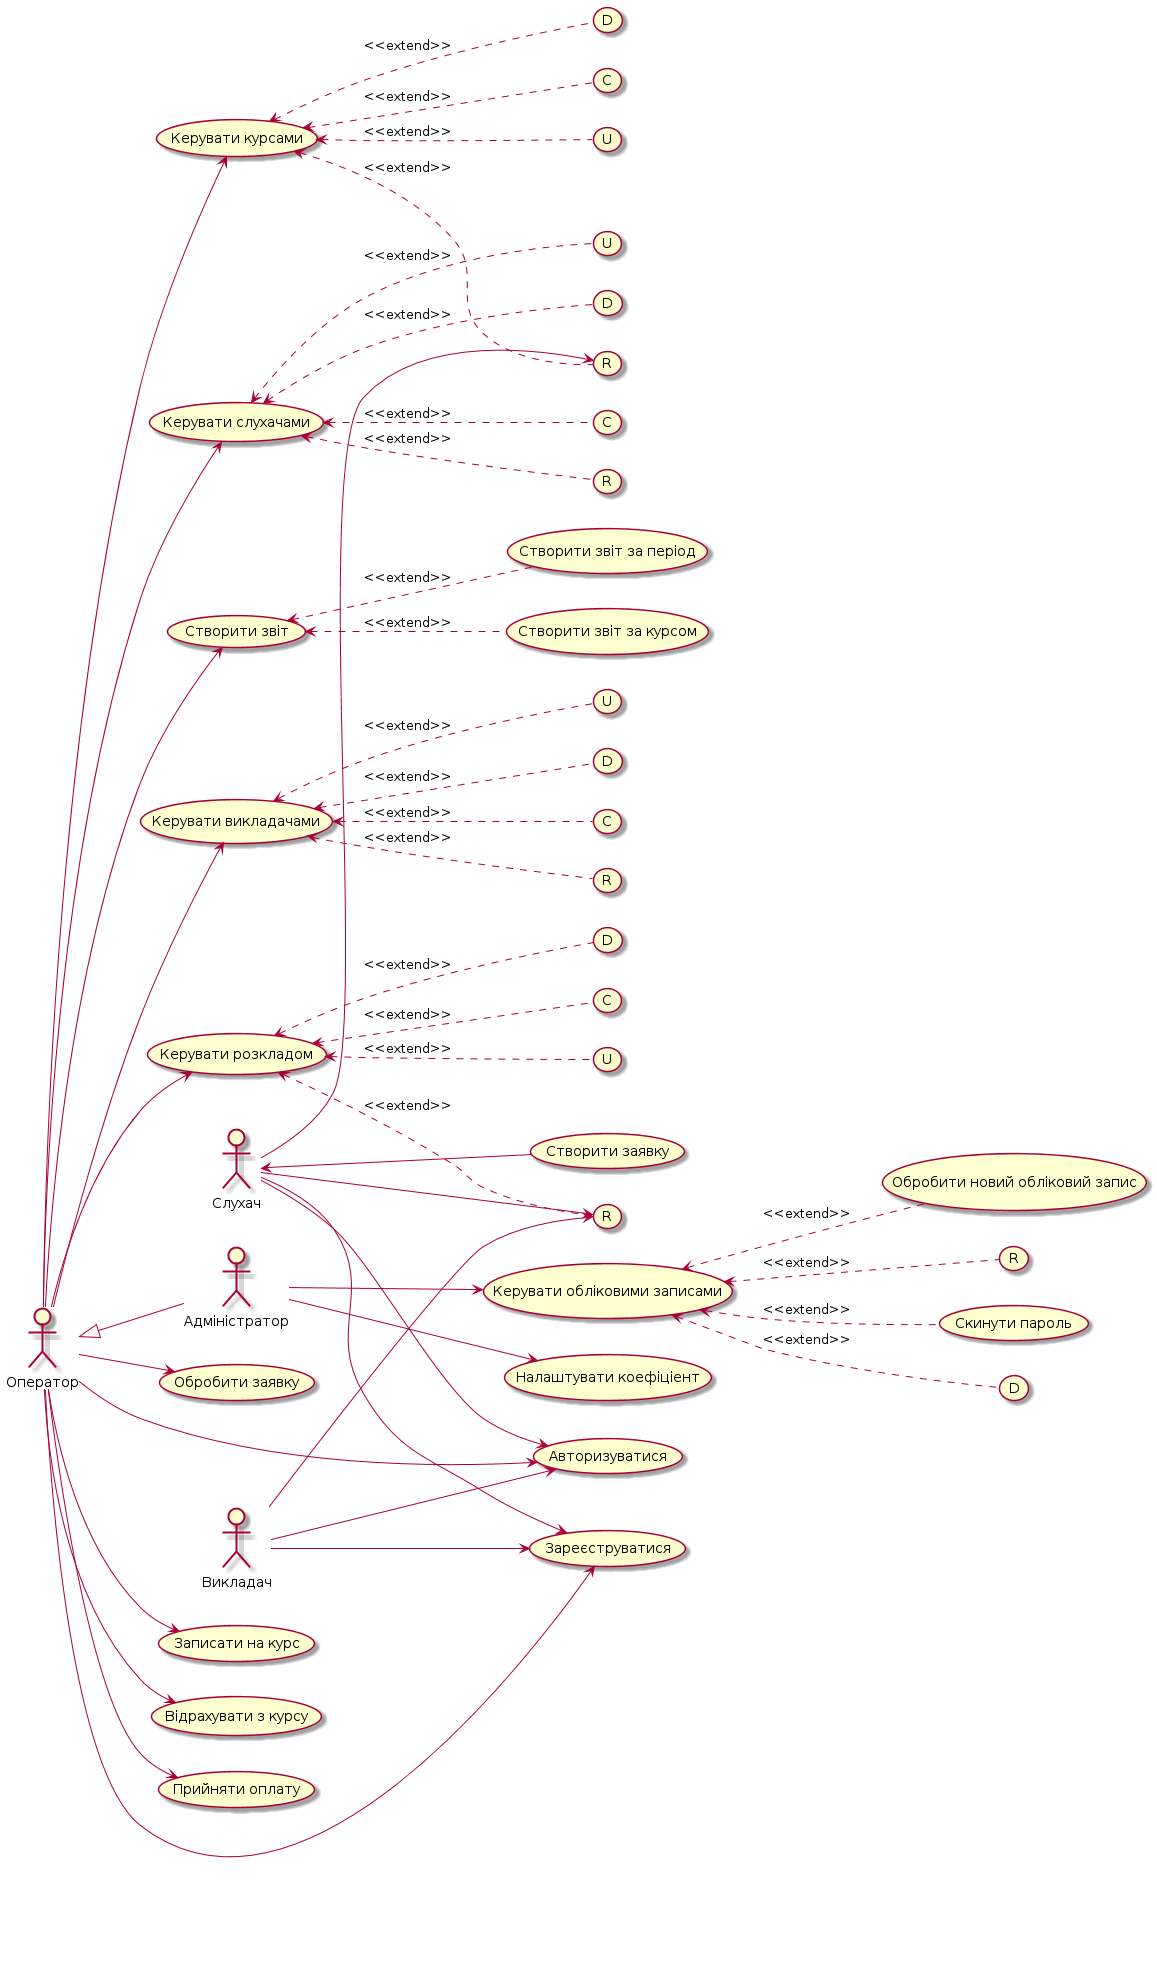
\includegraphics[width=14cm]{pp_pw1_uc.png}
\addimglabel{А}{Діаграма варіантів використання}

\begin{landscape}
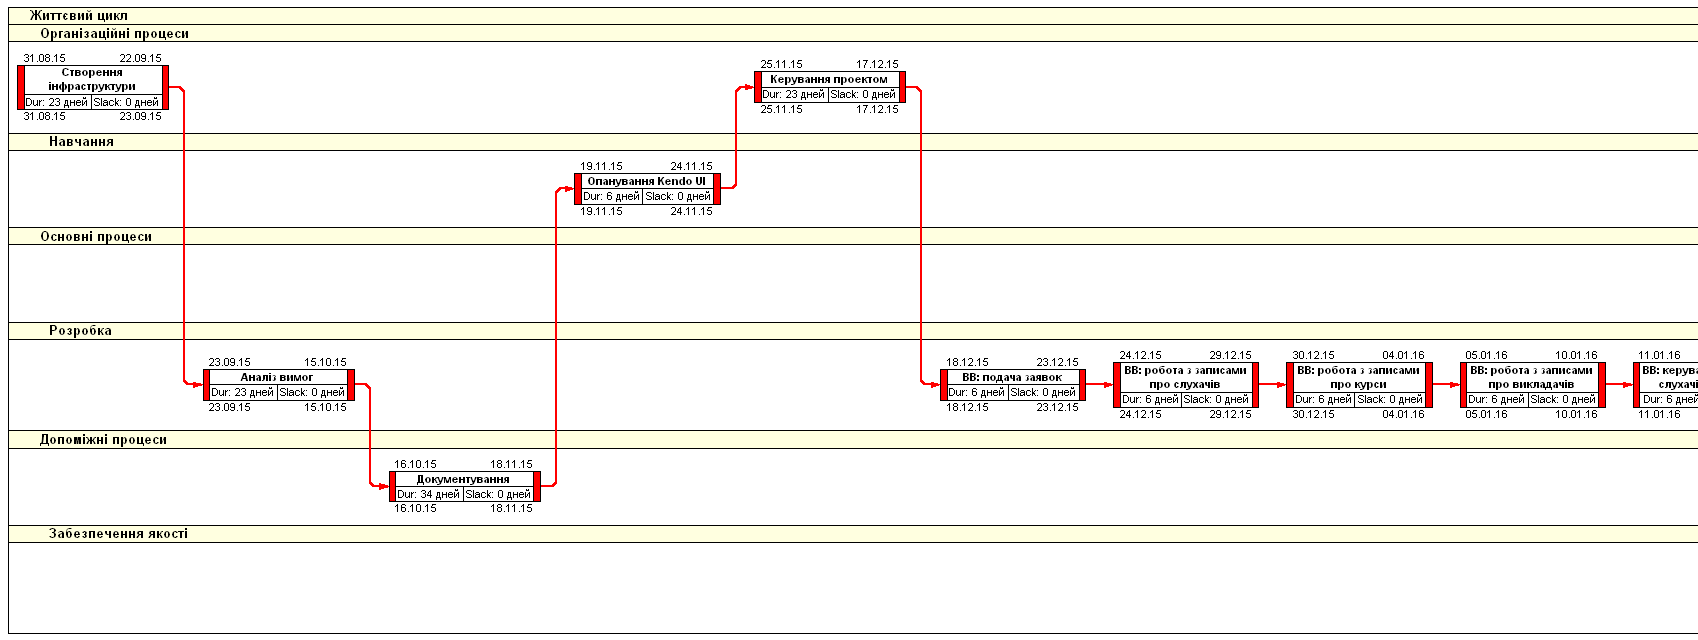
\includegraphics[width=24cm]{smp_cgw2_2.png}\\
\addpolyimglabel{А}{Діаграма WBS}{1}
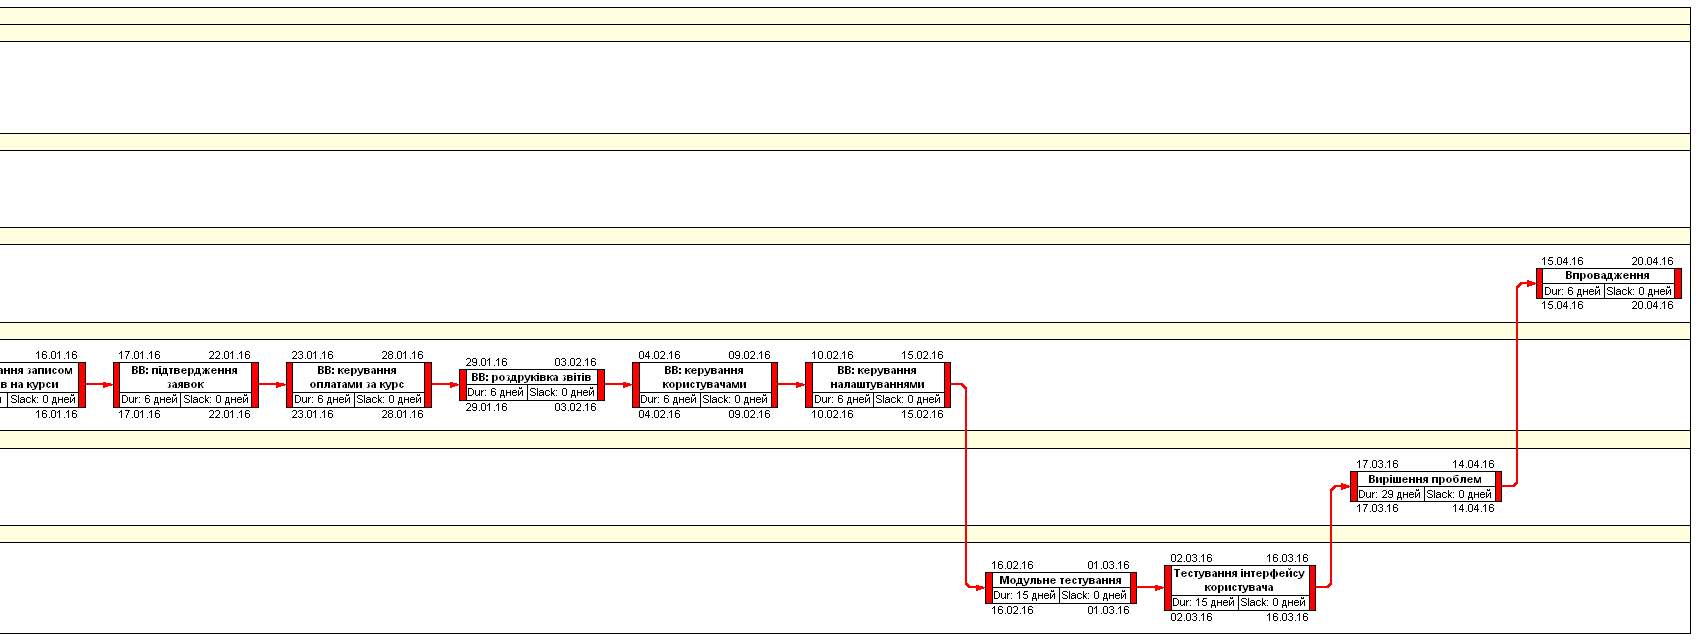
\includegraphics[width=24cm]{smp_cgw2_3.png}\\
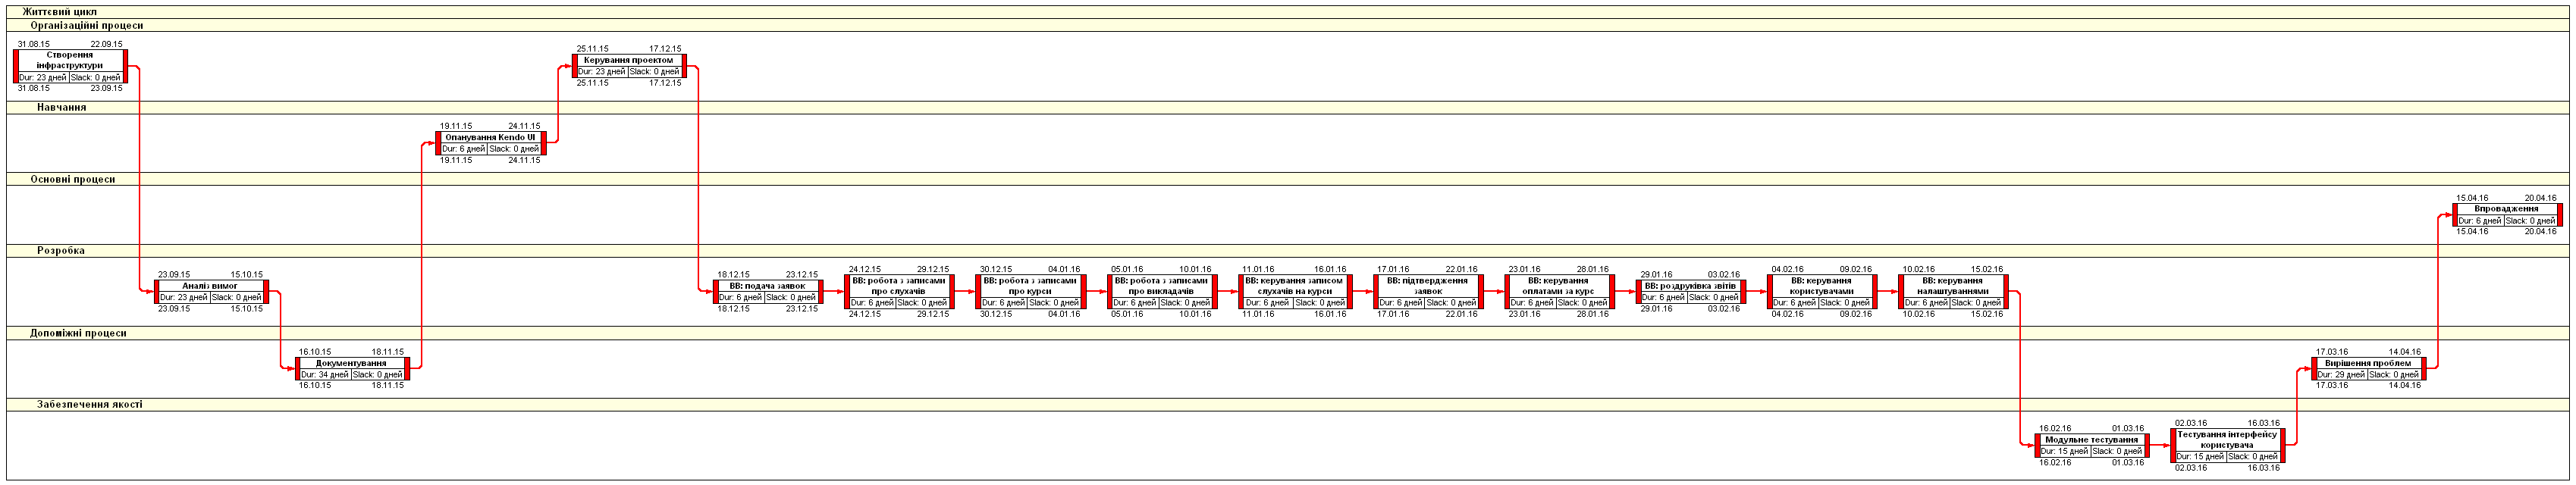
\includegraphics[width=24cm]{smp_cgw2_4.png}
\addtocounter{imgcount}{-1}
\addpolyimglabel{А}{Діаграма WBS}{2}
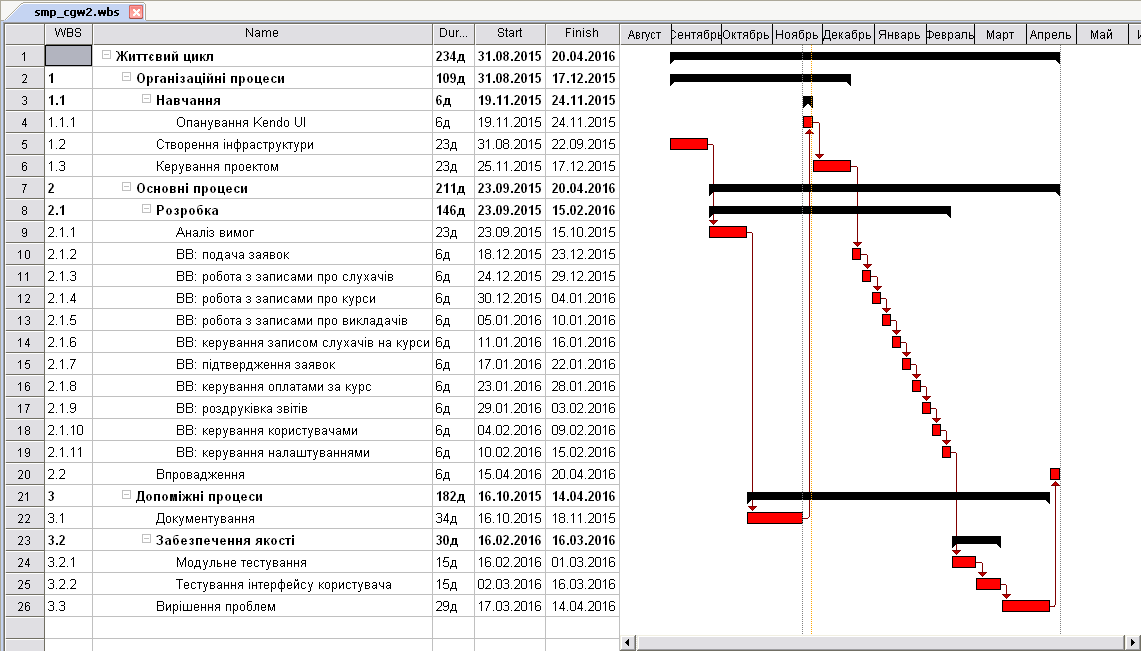
\includegraphics[width=24cm]{smp_cgw2_1.png}
\addimglabel{А}{Діаграма Ганта}
\end{landscape}

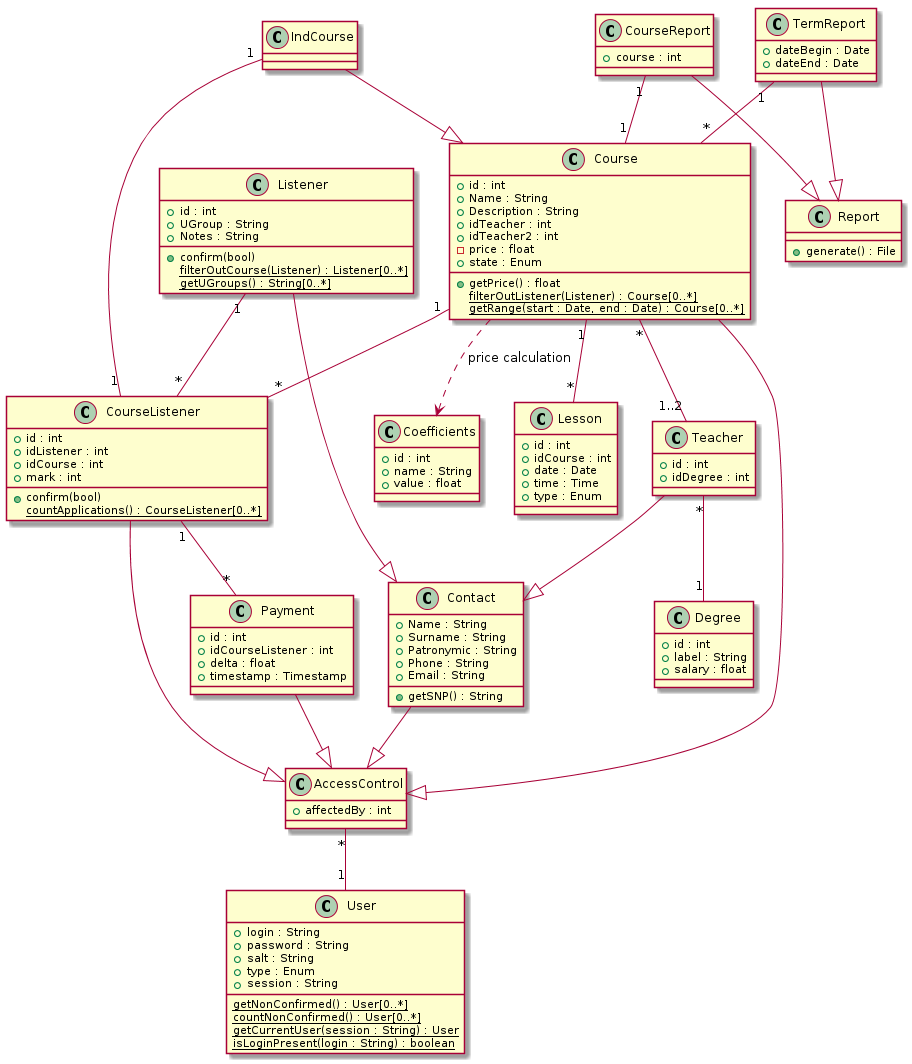
\includegraphics[width=17cm]{pp_pw3_clas.png}
\addimglabel{А}{Діаграма програмних класів}

\newpage
\tikzset{
	line/.style={draw, -latex'},
	every join/.style={line},
	u/.style={anchor=south},
	r/.style={anchor=west},
	fxd/.style={text width = 6em},
	it/.style={font={\small\itshape}},
	bf/.style={font={\small\bfseries}}
}
\tikzstyle{base} =
	[
		draw,
		on chain,
		on grid,
		align=center,
		minimum height=4ex,
		minimum width = 10ex,
		node distance = 6mm and 60mm,
		text badly centered
	]
\tikzstyle{coord} =
	[
		coordinate,
		on chain,
		on grid
	]
\tikzstyle{cloud} =
	[
		base,
		ellipse,
		fill = red!5,
		node distance = 3cm,
		minimum height = 2em
	]
\tikzstyle{decision} =
	[
		base,
		diamond,
		aspect=2,
		fill = green!10,
		node distance = 2cm,
		inner sep = 0pt
	]
\tikzstyle{block} =
	[
		rectangle,
		base,
		fill = blue!3,
		rounded corners,
		minimum height = 2em
	]
\tikzstyle{print_block} =
	[
		base,
		tape,
		tape bend top=none,
		fill = yellow!10
	]
\tikzstyle{io} =
	[
		base,
		trapezium,
		trapezium left angle = 70,
		trapezium right angle = 110,
		fill = blue!5
	]
\makeatletter
\pgfkeys{/pgf/.cd,
	subrtshape w/.initial=2mm,
	cycleshape w/.initial=2mm
}
\pgfdeclareshape{subrtshape}{
	\inheritsavedanchors[from=rectangle]
	\inheritanchorborder[from=rectangle]
	\inheritanchor[from=rectangle]{north}
	\inheritanchor[from=rectangle]{center}
	\inheritanchor[from=rectangle]{west}
	\inheritanchor[from=rectangle]{east}
	\inheritanchor[from=rectangle]{mid}
	\inheritanchor[from=rectangle]{base}
	\inheritanchor[from=rectangle]{south}
	\backgroundpath{
		\southwest \pgf@xa=\pgf@x \pgf@ya=\pgf@y
		\northeast \pgf@xb=\pgf@x \pgf@yb=\pgf@y
		\pgfmathsetlength\pgfutil@tempdima{\pgfkeysvalueof{/pgf/subrtshape w}}
		\def\ppd@offset{\pgfpoint{\pgfutil@tempdima}{0ex}}
		\def\ppd@offsetm{\pgfpoint{-\pgfutil@tempdima}{0ex}}
		\pgfpathmoveto{\pgfqpoint{\pgf@xa}{\pgf@ya}}
		\pgfpathlineto{\pgfqpoint{\pgf@xb}{\pgf@ya}}
		\pgfpathlineto{\pgfqpoint{\pgf@xb}{\pgf@yb}}
		\pgfpathlineto{\pgfqpoint{\pgf@xa}{\pgf@yb}}
		\pgfpathclose
		\pgfpathmoveto{\pgfpointadd{\pgfpoint{\pgf@xa}{\pgf@yb}}{\ppd@offsetm}}
		\pgfpathlineto{\pgfpointadd{\pgfpoint{\pgf@xa}{\pgf@ya}}{\ppd@offsetm}}
		\pgfpathlineto{\pgfpointadd{\pgfpoint{\pgf@xb}{\pgf@ya}}{\ppd@offset}}
		\pgfpathlineto{\pgfpointadd{\pgfpoint{\pgf@xb}{\pgf@yb}}{\ppd@offset}}
		\pgfpathclose
	}
}
\pgfdeclareshape{cyclebegshape}{
	\inheritsavedanchors[from=rectangle]
	\inheritanchorborder[from=rectangle]
	\inheritanchor[from=rectangle]{north}
	\inheritanchor[from=rectangle]{center}
	\inheritanchor[from=rectangle]{west}
	\inheritanchor[from=rectangle]{east}
	\inheritanchor[from=rectangle]{mid}
	\inheritanchor[from=rectangle]{base}
	\inheritanchor[from=rectangle]{south}
	\backgroundpath{
		\southwest \pgf@xa=\pgf@x \pgf@ya=\pgf@y
		\northeast \pgf@xb=\pgf@x \pgf@yb=\pgf@y
		\pgfmathsetlength\pgfutil@tempdima{\pgfkeysvalueof{/pgf/cycleshape w}}
		\pgfpathmoveto{\pgfqpoint{\pgf@xa}{\pgf@ya}}
\pgfpathlineto{\pgfpointadd{\pgfpoint{\pgf@xa}{\pgf@yb}}{\pgfpoint{0ex}{-\pgfutil@tempdima}}}
\pgfpathlineto{\pgfpointadd{\pgfpoint{\pgf@xa}{\pgf@yb}}{\pgfpoint{\pgfutil@tempdima}{0ex}}}
\pgfpathlineto{\pgfpointadd{\pgfpoint{\pgf@xb}{\pgf@yb}}{\pgfpoint{-\pgfutil@tempdima}{0ex}}}
\pgfpathlineto{\pgfpointadd{\pgfpoint{\pgf@xb}{\pgf@yb}}{\pgfpoint{0ex}{-\pgfutil@tempdima}}}
\pgfpathlineto{\pgfqpoint{\pgf@xb}{\pgf@ya}}
		\pgfpathclose
	}
}
\pgfdeclareshape{cycleendshape}{
	\inheritsavedanchors[from=rectangle]
	\inheritanchorborder[from=rectangle]
	\inheritanchor[from=rectangle]{north}
	\inheritanchor[from=rectangle]{center}
	\inheritanchor[from=rectangle]{west}
	\inheritanchor[from=rectangle]{east}
	\inheritanchor[from=rectangle]{mid}
	\inheritanchor[from=rectangle]{base}
	\inheritanchor[from=rectangle]{south}
	\backgroundpath{
		\southwest \pgf@xa=\pgf@x \pgf@ya=\pgf@y
		\northeast \pgf@xb=\pgf@x \pgf@yb=\pgf@y
		\pgfmathsetlength\pgfutil@tempdima{\pgfkeysvalueof{/pgf/cycleshape w}}
		\pgfpathmoveto{\pgfqpoint{\pgf@xb}{\pgf@yb}}
\pgfpathlineto{\pgfpointadd{\pgfpoint{\pgf@xb}{\pgf@ya}}{\pgfpoint{0ex}{\pgfutil@tempdima}}}
\pgfpathlineto{\pgfpointadd{\pgfpoint{\pgf@xb}{\pgf@ya}}{\pgfpoint{-\pgfutil@tempdima}{0ex}}}
\pgfpathlineto{\pgfpointadd{\pgfpoint{\pgf@xa}{\pgf@ya}}{\pgfpoint{\pgfutil@tempdima}{0ex}}}
\pgfpathlineto{\pgfpointadd{\pgfpoint{\pgf@xa}{\pgf@ya}}{\pgfpoint{0ex}{\pgfutil@tempdima}}}
\pgfpathlineto{\pgfqpoint{\pgf@xa}{\pgf@yb}}
		\pgfpathclose
	}
}
\makeatother
\tikzstyle{subroutine} =
	[
		base,
		subrtshape,
		fill = green!25
	]
\tikzstyle{cyclebegin} =
	[
		base,
		cyclebegshape,
		fill = blue!25
	]
\tikzstyle{cycleend} =
	[
		base,
		cycleendshape,
		fill = blue!25
	]
\tikzstyle{connector} =
	[
		base,
		circle,
		fill = red!25,
		minimum width = 3mm
	]

\begin{center}
{ \fontsize{12pt}{14pt} \selectfont
\begin{tikzpicture}[%
    start chain=going below,
    node distance=5mm and 60mm,
        ]
        \node [cloud] (start) {getCoursePrice(id, full)};
	\node [block, join] (global) {PRICE\_TRUNK := 10};
	\node [block, join] (q1) {price := вартість з таблиці courses\\для курсу id,};
	\node [decision, join] (q1cond) {price = 0};
	\node [block, join] (q2) {count := кількість слухачів\\з таблиці Course\_Listeners\\для курсу id};
	\node [block, join] (q3) {salary := (зарплата з таблиці prices\\для вченого ступеню з таблиці teachers\\для викладача з таблиці courses) *\\(кількість занять з таблиці lessons\\з типом <<Лекція>>) + (зарплата з таблиці prices\\для вченого ступеню з таблиці teachers\\для другого викладача з таблиці courses) *\\(кількість занять з таблиці lessons\\з типом <<Практика>>)};
        \node [subroutine, join, subrtshape w = 3mm, fxd] (coefficients) {coef := getCoefficients()};
	\node [block, join] (price) {price := $\left[ \frac{salary \cdot coef.personal \cdot coef.bonus \cdot coef.others}{count \cdot PRICE\_TRUNK}\right] \cdot PRICE\_TRUNK$};
	\node [decision, join] (fullcond) {full};
	\node [block] (fullmul) {price := $price \cdot count$};
        \node [cloud, join] (finish) {Повернення price};

        \path [line] (q1cond) to node [r] {Так} (q2);
        \path [line] (q1cond) -- node [u,near start] {Ні} ++(7cm, 0cm) |- (finish);
        \path [line] (fullcond) to node [r] {Так} (fullmul);
        \path [line] (fullcond) -- node [u,near start] {Ні} ++(3cm, 0cm) |- (finish);
\end{tikzpicture}
}
\end{center}
\addimglabel{А}{Алгоритм розрахунку вартості курсу}
\begin{center}
{ \fontsize{12pt}{14pt} \selectfont
\begin{tikzpicture}[%
    start chain=going below,
    node distance=5mm and 60mm,
        ]
        \node [cloud] (start) {user\_login(login, pass)};
	\node [block, join] (config) {config := з файлу конфігурації};
	\node [block, join] (q1) {user[password, salt, sessionid] := з\\таблиці users для логіну login};
	\node [decision, join] (q1cond) {user = $\emptyset$};
	\node [decision, yshift=-3mm] (confcond) {sessionid = <<q>>};
	\node [block] (crypt) {hash := crypt(pass,\\config.global\_salt)};
	\node [decision, join] (passcond) {pass = hash};
	\node [block] (gensess) {sess\_id := randhash(login, 500)};
	\node [block, join] (updsess) {Встановити в\\таблиці users\\sessionid := sess\_id\\для логіну login};
	\node [block, join] (cookiesess) {Записати sess\_id в Cookies};
	\node [block, join] (gotomain) {Перейти на головну сторінку};
        \node [cloud, join] (finish) {Вихід};

	\node [block, right of = q1cond, node distance = 8.5cm, yshift = -5mm] (err5) {Помилка 400:\\користувача не знайдено};
	\node [block, right of = confcond, node distance = 6.2cm, yshift = -5mm] (err10) {Помилка 403:\\обліковий запис\\ще не підтверджено};
	\node [block, right of = passcond, node distance = 4.5cm, yshift = -5mm] (err6) {Помилка 403:\\пароль невірний};

        \path [line] (q1cond) to node [r] {Ні} (confcond);
        \path [line] (q1cond) -| node [u,near start] {Так} (err5);
        \path [line] (err5) |- node {} (finish);
        \path [line] (confcond) to node [r] {Ні} (crypt);
        \path [line] (confcond) -| node [u,near start] {Так} (err10);
        \path [line] (err10) |- node {} (finish);
        \path [line] (passcond) to node [r] {Так} (gensess);
        \path [line] (passcond) -| node [u,near start] {Ні} (err6);
        \path [line] (err6) |- node {} (finish);
\end{tikzpicture}
}
\end{center}
\addimglabel{А}{Алгоритм аутентифікації та авторизації}
